\chapter{Experiment 2 - Malware Dataset Transformation}
\label{chap:three}
% Introduction
Neural networks have demonstrated some success in the security domain~\cite{raff2018malware} and so we have applied neural networks to the Watkins~\cite{watkins2013using} dataset.
Briefly, this dataset consists of interarrival times for packets sent to Android devices, some of which were running malware.
Detecting malware via network traffic is an important problem, and this interpretation of the problem is crucial for addressing the situation where a device which is infected with malware is outside of the network owner's control.
This is a common situation when personal devices are introduced to a corporate network, and so being able to detect malicious software on a device without having an agent on the device provides a tremendous benefit to network defenders.

\section{Data}
For our experiment, we leveraged four different datasets whose summary statistics are in Table~\ref{Tab:summary}. 
Our data consisted of 98 legitimate applications and 120 pieces of malware, which were collected by Yu and Li~\cite{yu2018network}.
This gives us a dataset which is approximately 55\% malware and 45\% benignware.
While this distribution is not reflective of real environments where malware is significantly rarer than benign applications, we do not adjust for this disparity since our tolerance for alerting on benign applications is much higher than our tolerance for not detecting malicious applications. 
For each application, 5 trials were conducted where the interarrival time was collected for each of 100 ICMP ping packets.
Further details of the data collection can be found in \cite{yu2018network, watkins2013using}

\subsection{Raw data}
This is the data as described above, captured by Yu and Li in accordance with Watkins~\cite{watkins2013using}.
In this dataset, only the raw measurements are used in a 100-dimensional row vector, with a label of 0 for benign and 1 for malicious.

\subsection{Summary data}
The summary data leverages the seven features used by Yu and Li: arithmetic mean, standard deviation, variance, maximum, minimum, geometric mean, and harmonic mean. 
These features were fed to the classifier based on the sample they were captured from as a 7-dimensional row vector.

\subsection{Fourier data}
This dataset is a copy of the raw data under the Fourier transform.
In particular, since our raw data is given by a single 100-dimensional row vector, it is a direct mapping of that row vector under the Fast Fourier Transform as provided by the numpy library.

\subsection{Wavelet data}
The wavelet dataset is a copy of the raw data under a continuous wavelet transform. 
The Morlet wavelet is used for the transform for several reasons:
First, it is a wavelet which allows us to maintain the dimensionality of our data, making it easier to compare in performance and to re-use neural network architectures.
Secondly, the Morlet wavelet is closely related to human perception~\cite{mallat1999wavelet, daugman1985uncertainty}, providing a small connection to the human brain conception of neural networks.
Lastly, the Morlet wavelet is uniquely invertible, which is not the case for all potential mother wavelets. 
Since both detail and approximation coefficients are produced by the wavelet transform, but the detail coefficient-only results were identical to the results where both were used in all trials, the two-channel data was used.
This likely relates to the volume of high-frequency parameters in the parameter space~\cite{rahaman2018spectral} and the vanishing gradients experienced by the low-pass approximation coefficient values close to zero.
Further investigation of the density of information in different bands of the signal has been considered by de Oliveira \textit{et al.}~\cite{de2006wavelet} but is outside the scope of this document.

One interesting effect of performing the transforms on the dataset is that while the continuous wavelet transform reduces our variance significantly and slightly normalizes the dataset, the Fourier transform has the opposite effect, introducing tremendous amounts of noise into the dataset.
Given our results in \ref{invariance}, we would expect this not to have a meaningful impact on the accuracy, though increased variance is likely to have an impact on time to convergence.

\renewcommand{\thefootnote}{*} 
\begin{table}[h]
\centering
\label{Tab:summary}	
\begin{tabular}{l|llll}
\textbf{Dataset Name} & \textbf{Mean} & \textbf{Median} & \textbf{Mean Var.} & \textbf{Median Var.} \\\cline{1-5}
Raw         & 27.43    & 10.07    & 8329.96    & 7663.89 \\
Fourier       & 58.60\footnotemark    & -1.45    & 12229005.34    & 7418186.12 \\
Wavelet        & 1.30    & -.072    & 1887.5    & 1507.16 \\             
\end{tabular}
\caption{Dataset Summary Statistics}
\end{table}
\footnotetext{There is an extremely small, but non-zero imaginary part, on the order of $10^{-19}i$}

\renewcommand{\thefootnote}{1}
It is worth noting that the small but non-zero imaginary part in the Fourier data required implementation of methods from Trabelsi \textit{et al.}~\cite{trabelsi2017deep} to achieve acceptable results.

\section{Models}
For each of the aforementioned datasets, with the exception of the Summary Statistic dataset, we leveraged each of the following models:
\begin{itemize}
\item Fully Connected Neural Network
\item Convolutional Neural Network
\item Random Forest
\item Support Vector Classifier	
\end{itemize}

\subsection{Baseline Models} \label{other models}
Two baseline models were considered.
The first is the random forest model provided in the Scikit-learn library with no hyperparameter tuning.
Decision tree models are generally good at classification tasks~\cite{hastie01statisticallearning} but are weak classifiers which are sensitive to variance.
Random forests are a the result of averaging a large collection of de-correlated trees and provide a good benchmark as a na\"ive model - in the respect that it is untuned - for classification.

The other benchmark model is a Support Vector Classifier, again provided by the Scikit-learn library.
The rationale for using a Support Vector Machine is that we wanted to see if some hyperplane could be learned which would separate the data.
This model was again, na\"ive in the respect that it was merely the ``out of the box'' model, and so the classifier was built on top of the radial basis function kernel.

The summary statistic dataset was not used with the convolutional neural network because there is no spatial relationship between the data.
The architecture of the convolutional neural network is visualized below in figure \ref{fig:conv net}.

\begin{figure}[ht]
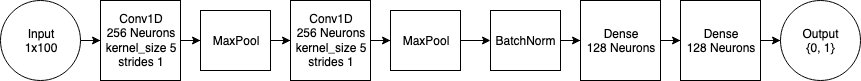
\includegraphics[width=\textwidth]{conv_architecture}
\centering
\caption{Convolutional Neural Network Architecture}
\label{fig:conv net}
\end{figure}


\section{Methodology and Results}
Hardware specifications on which these models ran is in \ref{append:one}.
In order to ensure that deviations in the dataset did not induce significant variation in accuracy, this experiment was run 100 times, and the accuracy and mean step time for all trials was averaged.

\begin{table}[h]
\centering
\label{Tab:test}	
\begin{tabular}{l|ll}
\textbf{Data and Architecture Combination} & \textbf{Test Accuracy} & \textbf{Mean Step Time} ($\mu$s) \\\cline{1-3}
Raw, Fully-Connected NN            & 63.40\%         & 13\\
Summary, Fully-Connected NN        & 55.14\%         & 13\\
Fourier, Fully-Connected NN        & 59.88\%         & 12\\
Wavelet, Fully-Connected NN        & 61.95\%         & 12\\
\hline
Raw, Convolutional NN              & 72.89\%         & 54\\
Fourier, Convolutional NN          & 70.81\%         & 56\\
Wavelet, Convolutional NN          & 70.77\%         & 52\\
\hline
Raw, Random Forest                 & 80.28\%         & N/A\\ 
Summary, Random Forest             & 76.91\%         & N/A\\
Fourier, Random Forest             & 79.63\%         & N/A\\
Wavelet, Random Forest             & 79.80\%         & N/A\\
\hline
Raw, Support Vector Classifier     & 65.77\%         & N/A\\    
Summary, Support Vector Classifier & 55.28\%         & N/A\\  
Fourier, Support Vector Classifier & 55.28\%         & N/A\\  
Wavelet, Support Vector Classifier & 55.28\%         & N/A           
\end{tabular}
\caption{Android App Data Test Results}
\end{table}

In terms of pure accuracy, we find that the random forest on the raw data gives us the best accuracy, followed closely by the random forest on the wavelet-transformed data, and third the random forest trained on the Fourier-transformed data. 
Notably, when we compare accuracy by model, we find that for the fully-connected neural network, our maximum average accuracy is 63.40\%, while our minimum average accuracy is given by the summary statistics.
Excluding the summary statistic data, the difference between the highest average accuracy and lowest average accuracy for fully-connected neural networks is 3.52\%, a very small margin. 
Comparatively, for the convolutional neural network, our delta is 2.12\%, again - quite small. 
Similarly, the random forest performs near the 80\% mark universally, irrespective of representation, and performs worst on the summary statistic dataset. 
